\documentclass{article}

\usepackage{header}

\begin{document}

\tableofcontents
\newpage

\section{unfiled lol make sure everything makes sense tho}
\subsection{Impedance Matching}

\begin{define}
    \textbf{Impedance:} the total resistance of a given electric component or AC circuit originating from reactive and resistance of the given system. Has both \textit{phase} and \textit{resistance} for AC. For DC, impedance has zero phase angle.

    \textbf{Impedance matching:} the process where the input impedance and the output impedance of a given electrical load are designed to reduce signal reflection and maximize the power transferred to the electric load.
\end{define}

\subsubsection{Motivation}
Impedance matching has great use in high-frequency and high-speed devices. 

When designing applications of ultra-high frequencies, impedance matching becomes a difficult operation for designers. The challenge is also reflected while designing microwaves and radio frequency circuits. When you get a wrong impedance matching, expect distorted pulses and high signal reflections.

An increase in frequency decreases the window of errors. The electrical circuit works the best when we have a perfectly matched impedance. If the impedance matching is not done, expect the system to work abnormally because of the effects such as the signal reflections. The reflected waves cause data delays and distortion of the phase and minimize the ratio of signal to noise.

\begin{concept}
    Maximum power transfer occurs when the resistance of the voltage source is equal to the resistance of the load.
\end{concept}

We can show this by taking the derivative of the power function. At maximum power transfer, this derivative is equal to zero
\subsubsection{Examples}
\begin{enumerate}
    \item Suppose that we have a system that is modeled by the circuit below
    \begin{center}
        \begin{circuitikz}[american]
            \draw (0,0)
            to[V, v=$V$, invert] (0,2)
            to[R, l=$R_{in}$, i=$i_{load}$] (2,2)
            to[R, l=$R_{load}$] (2,0)
            -- (0,0);
            \draw (2,2) -* (4,2) to[open, v=$V_{\text{out}}$] (4,0) -- (2,0);
        \end{circuitikz}    
    \end{center}
    \begin{align*}
        P &= I_{load}^2 R_{load} = \frac{V^2 R_{load}}{(R_{in} + R_{load})^2} \\
        \frac{dP}{dR_{load}} &= \frac{V^2(R_{in} + R_{load})^2 - 2R_{load}(R_{in} + R_{load})V^2}{(R_{in} + R_{load})^4} = 0 \Rightarrow R_{load} = R_{in}
    \end{align*}

    \item Suppose now you have the following circuit
        \begin{center}
            \begin{circuitikz}
                \draw (0,0)
                to[C, l=$C$] ++(0,2)
                to[L, l=$L$] ++(3,0)
                to[R, l=$R$] ++(0,-2)
                to (0,0);
            \end{circuitikz}
        \end{center}
        The admittance of the circuit, $Y_{in}$ is the inverse of the impedance. Here are the general steps for finding some $R'$ and $R$ such that their impedances matched
        \begin{enumerate}
            \item Calculate the impedance $Z$ of the circuit.
            \item Set admittance $Y = \frac{1}{Z}$.
            \item Separate your admittance into its real and imaginary part to take the real part of $Y$.
            \item $R' = \Re\{Y\}$, so that $R'$ here is a function of $R$.
        \end{enumerate}

    \textcolor{red}{i dont feel like doing the calculations right now im too tired do later though : \href{https://eepower.com/technical-articles/understanding-impedance-matching}{link}}

    \item \textbf{Transformer impedance matching:} set the turn ratio accordingly. Low voltage $\rightarrow$ fewer turns. 
        \begin{define}
            \[\text{Turns ratio }= \sqrt{\frac{\text{Source resistance}}{\text{Load resistance}}}\]
        \end{define}
    
    \item \textbf{Transmission line:} Transmission of electrical energy from the source to the load is done using a transmission line. While transferring this energy, it is important to zero or minimize energy losses that occur. For this to be possible, we should match the source and load impedances to the transmission line being used.
    
    The characteristic impedance is defined as the voltage and current wave ratio at any given point along the transmission line. If the transmission line in discussion is long, then we expect to have a different characteristic impedance at different distances along this transmission line. If we fail to do the impedance matching, the signs reaching the load will be reflected in the source of the origin, giving rise to a standing wave. The amount of power reflected is measured using the coefficient of reflection, which is calculated using the equation below
        \begin{define}
            \[\Gamma  = \frac{Z_L - Z_0}{Z_L + Z_0}\]
            $Z_L$: line impedance, $Z_0$: characteristic impedance
        \end{define}

    \item Attenna and television
        \begin{center}
            \begin{circuitikz}
                \draw (0,0)
                to[sV, v=$V_{in}$] ++(0,2)
                to[R, l=$R_A$] ++(3,0)
                to[R, l=$R_L$] ++(0,-2)
                to (0,0);
            \end{circuitikz}
        \end{center}
        $R_A$ is the resistance of the antenna is 150$\Omega$ and its cable while the TV's resistance is 600$\Omega$. Use the turns ratio formula to find the number of turns. Then set a transformer in between like in the image below.
        \begin{figure}[H]
            \centering
            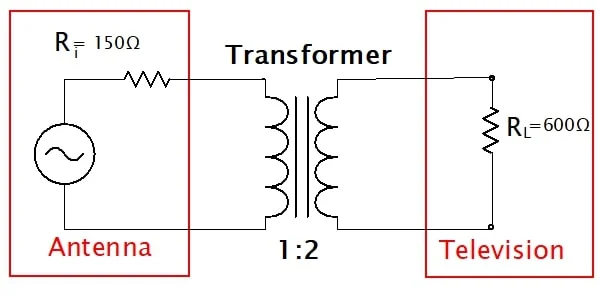
\includegraphics[scale=0.8]{figs/z_match_ex5.png}
        \end{figure}

    \item In the case of the headphone, the signal source is the device where the headphone is plugged. The headphone is the load. For the system to attain quality audio output, the source, and the load impedances must be matched. By matching the impedances, we make sure that there is maximum power transfer from the source of the audio to the headphone.

    When building portable devices, ensure that low-impedance headphones are built. This makes the system work well with proper sound quality.
\end{enumerate}




\section{Introduction to Power}
What is Power Electronics?

\begin{define}
\textbf{Source:} something that generates power

\textbf{Load:} something that consumes power

\textbf{Power electronics:} application of electronics and circuitry to control the conversion of one form to another
\end{define}

Converter types between AC and DC Power: DC stands for "direct current" and can be visualized as a constant voltage over time. One example is a battery and photovoltaic panel. AC power stands for "alternating current" and is a sinusoidal voltage in time. An example of this is the power from the outlet. There are four basic types of converters.
\begin{itemize}
    \item AC-DC: AC source to DC load, which is commonly called a rectifier like in the use of a laptop charger
    \item DC-DC: DC source to DC load, battery pack USB
    \item DC-AC: DC source to AC load, also commonly called an inverter like for a photovoltaic to grid system
    \item AC-AC: AC source to AC load, not as common but used in wond power system
\end{itemize}

\subsection{Average and Root Mean Square (RMS) Calculations}
Period waveforms repeat their shape across each period. The average value of a sine wave is 0. $\langle v(t) \rangle = \frac{1}{T} \int_0^T v(t) \,dt$ will represent the average value here.

The RMS is represented as capital V listed below
\begin{define}
    \[V = \sqrt{\frac{1}{T} \int_0^T v(t)^2 \,dt}\]
\end{define}
We can think of the RMS value as the equivalent voltage if we put the waveform of choice across a resistor

The power is equal to the voltage waveform squared over the resistor. The triangle brackets represent the average here.
\begin{define}
    \[\langle P \rangle = \langle \frac{v^2}{R} \rangle = v^2\]
\end{define}
Remember that 
\[\langle v \rangle ^2 \neq v^2\]

If we take a look at this sine wave and say that this represents current and connected this to a resistor, average power would not be 0 even though average current is 0. $I(t)$ here represents the instantaneous value. The resistor generates (consumes) power at both the negative and positive parts of this waveform.
\begin{center}
    \begin{tikzpicture}
        % Axes
        \draw[->] (0,0) -- (6.5,0) node[right] {$t$};
        \draw[->] (0,-1.5) -- (0,1.5) node[above] {$I(t)$};
        
        % Sine wave
        \draw[domain=0:2*pi,smooth,variable=\x,blue] plot ({\x},{sin(\x r)});
        
        % Labeling
        \draw[dashed] (pi/2,0) -- (pi/2,1) node[pos=0.5, right] {$\frac{\pi}{2}$};
        \draw[dashed] (3*pi/2,0) -- (3*pi/2,-1) node[pos=0.5, left] {$\frac{3\pi}{2}$};
        
        % Axes labels
        \node[below] at (pi,0) {$\pi$};
        \node[below] at (2*pi,0) {$2\pi$};
        \node[left] at (0,1) {1};
        \node[left] at (0,-1) {-1};
    \end{tikzpicture}
\end{center}

\begin{sanity}
    Is the RMS value always greater than or equal to the average value? Yes. Recall the definitions of average value and the RMS value above. My intuition behind this is that you're squaring a periodic function there will be no negative values.
\end{sanity}

Sine wave RMS value calculations:

Define $x(t) = X_{peak} \sin{(t \times \frac{2\pi}{T})}$. We multiply $t$ by a factor of $\frac{2\pi}{T}$ since we are working in units of time.
\begin{align*} 
    X_{RMS} &= \sqrt{\frac{1}{T} \int_0^T X_{peak}^2 \sin^2{(t \times \frac{2\pi}{T})} \,dt} \tag{1} \\
    &= \sqrt{\frac{X_{peak}^2}{T} \int_0^T (1-\cos{(2\cdot \frac{2\pi}{T})}) \,dt} \tag{2} \\
    &= \sqrt{\frac{X_{peak}^2}{2T} \left[t \mid_0^T - \sin{(\frac{4\pi t}{T})\frac{T}{4\pi} \mid_0^T}\right]_0^T} \tag{3} \\ 
    &= \sqrt{\frac{X_{peak}^2}{2T} \left[T - \frac{T}{4\pi}(\sin{(4\pi) - \sin{(0))}}\right]_0^T} \tag{4} \\
    &= \frac{X_{peak}}{\sqrt{2}} \tag{5}
\end{align*}

Line (2) comes from the trig idenity 
\[\sin^2{u} = \frac{1-\cos{(2u)}}{2}\]
Line (3) comes from evaluating the integral. In line (4), we see that everything within the brackets evaluates to $T$ and that this results in $T$ cancelling out with the $T$ in the denominator, resulting in just a 2 in the denominator, which is later square rooted.

\subsubsection{$X_{peak}$ and Oscilloscope Readings}
We notice that $X_{peak}$ is described in its RMS value as the large value that we can get. The amplitude of this sine wave is 1, but if we were to output this sinusoid in High-Z mode on the function generator, we would have to set this to a 2 $V_{pp}$ (Volt peak to peak). Contrastingly, if we were in 50-Ohm mode, setting the function generator to 2 $V_{pp}$ would result in a sinusoid with an $X_{peak}$ of 4 $V$.

Why is my function generator's output voltage wrong?
\begin{enumerate}
    \item \textbf{Scope vertical scale is using wrong probe attenuation.} A lot of scopes set this vertical scale automatically for you, so you may have to set this scale to be larger or smaller depending on how large your voltage is.
    \item \textbf{Load impedance is different from what the generator expects.} Image a voltage divider below. If our function generator wants to output 1 $V_{pp}$ at $R_{load}$ then, if $R_f = 50 \Omega$ and it assumes the $R_{load}$ is also $50 \Omega$ then that means thats the function generation will set $V_s$ as $2 V_{pp}$. However, sometimes it is the case that if $R_{load}$ is too high (such as in the case of the oscilloscope itself) then that means that voltage drop across $R_f$ is not that big and most of the voltage drop occurs across $R_f$. This results in us reading 2 $V_{pp}$ when we meant to output 1 $V_{pp}$. To correct this, correct the load impedance on the function generator settings if you have the setting for it to High-Z or what your load impedance on whatever you're connecting to is or connect a 50 $\Omega$ through terminator to your coax on your lead.
    \begin{center}
        \begin{circuitikz}[american]
            \draw (0,0) to[sinusoidal voltage source, v=$V_{\text{s}}$] (0,-2);
            \draw (0,0) to[R, l=$R_{f}$, v=$V_1$] (3,0);
            \draw (3,0) to[R, l=$R_{load}$, v=$V_2$] (3,-2);
            \draw (0,-2) -- (3,-2);
            \draw (3,0) -- (4,0) node[right] {$V_{\text{out}}$};
        \end{circuitikz}
    \end{center}
\end{enumerate}

\subsection{Real, Reactive and Apparent Power}
There are three different types of AC power. $\phi$ here is the impedance phase angle between the voltage and the current.
\begin{define}
    \textbf{Apparent power:} product of the RMS current and RMS voltage and represented by S in units of VA
    \[S = V_{RMS} I_{RMS}\]
    \textbf{Active/Real power:} power consumed or used within an AC circuit and represented by P. Is the real power in units of W (watts)
    \[P = V_{RMS} I_{RMS} \cos{\phi}\]
    \textbf{Reactive power:} the power developed in the circuit and represented by Q in units of VAR. Is the maximum value of the power component that "messes around", going back and forth
    \[Q = V_{RMS} I_{RMS} \sin{\phi}\]
\end{define}

We can describe the differences between apparent, reactive, and real power with a "sending a package analogy". The item you want to ship is your real power. To deliver power, you need a container, which is your apparent power. This has the potential to send an amount of power. However, you need some packaging in the container to cushion your item, which is your reactive power.
\begin{itemize}
    \item Real - item. Reactive loads like inductors and capacitors dissipate zero power
    \item Reactive - packaging. The actual amount of power being used or dissipated
    \item Apparent - box. This is the combination of reactive and real power and is without reference to phase angle.
\end{itemize}

\subsubsection{Pure Load Examples}


\begin{center}
    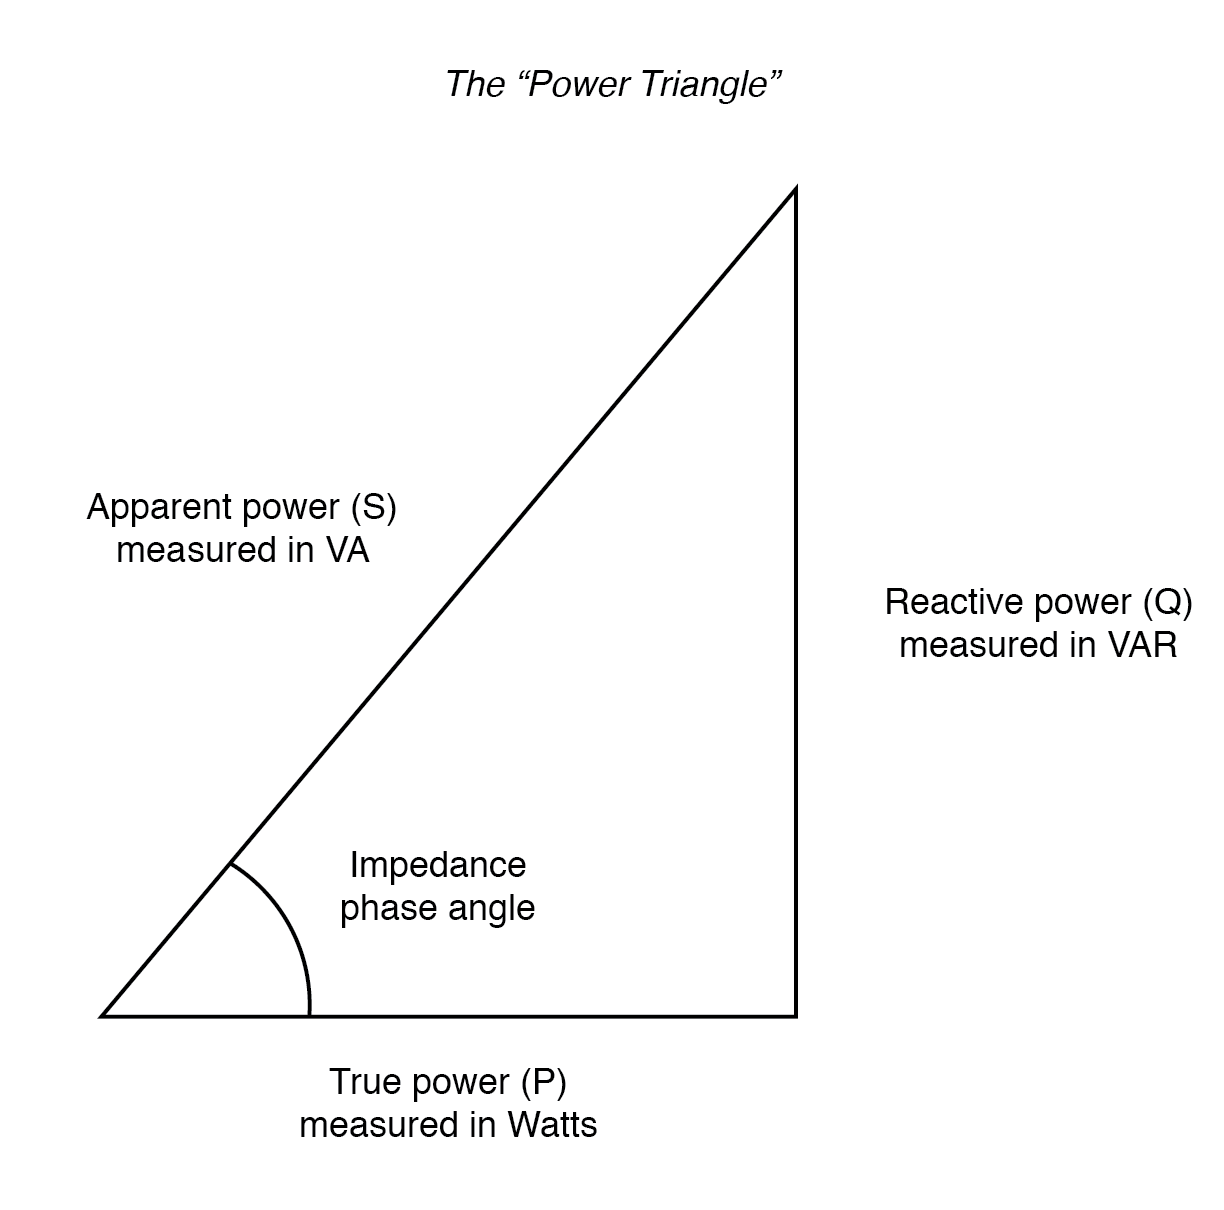
\includegraphics[scale=0.2]{figs/1_1_2_power_triangle.png}
\end{center}
\subsection{Power Factor}

\section{Power Converters}
Our switching converter is made

\section{Tranmission and Distribution}
\subsection{Three-phase Electric Power}
\begin{define}
    \textbf{Three-phase electric power:} a common type of alternating current (AC) used in electricity generation, transmission, and distribution. Typically employs 3-4 wires (fourth wire is an optional neutral return wire).

    \textbf{Line voltage:} the voltage between any two lines

    \textbf{Phase voltage:} the voltage measured between any line and neutral
\end{define}
This three-phase electric power is a common method used by electrical grids to transfer power. The voltage on each wire is 120$^\circ$ phase shifted from each other. This allows voltages to be stepped up using transformers to high voltage and stepped down for distribution. Each conductor in a \textit{symmetric} three-phase power supply system carries an alternating current of the same frequency and voltage amplitude. You can design assymetric three-phase power systems, but are not used in practice.

Convention states that for a 208/120-volt service, that means that the line voltage is 208 volts and the phase voltage is 120 volts.

\subsubsection{Advantages}
If we had to compare a three-phase supply to a single phase AC power supply (with two current-carrying conductors, phase and neutral), a three-phase supply with no neutral and the same phase-to-ground voltage/current capacity per phase would transmit 3 times as much power with only 1.5 imes as much wires (3 vs 2 wires). This means that we get higher efficiency, lower weight, and cleaner waveforms.

Here are more properties of three-phase supplies that are desirable in electric power systems:
\begin{itemize}
    \item Phase currents tend to cancel each other out, summing to 0 in a linear balanced load. Due to this, sometimes we don't even need a neutral conductor since it will carry little or no current.
    \item Power transfer into a linear balanced load is constant, which helps to reduce vibrations in motor/generators
    \item Can produce a rotating magnetic field with a specificed direction and constant magnitude. This simplifies the design of electric motors since no starting circuit is required
\end{itemize}

\subsubsection{Disadvantages or Cautions}
Make sure that the phases are connected in the correct order to achieve the intended direction of rotation of three-phase motors. If two sources are connected at the same time, then a direct connection between two different phases is a short circuit and leads to flow of unbalanced current.

\subsubsection{Why not a higher number of phases?}
Three phases is the minumum number that we can have without having "dead" spots in the cycle.

Industry uses almost exclusively three phase power since an induction motor needs at least a three phase supply to start and run in a known direction. Single phase induction motors require lossy, unreliable, and expensive tricks to do the same (extra windings, lossy windings, speed sensitive switch, capacitors, etc).

The supply grid is based on three phase since that is the most efficient in terms of generation and delivery. Using a 9 phase grid for example would require running 9 wires for the entire distribution grid, not cost effective.

The higher order motors mentioned don't use line generated phases. Stepper motors use more phases for finer control. High order polyphase rectifiers are designed often with more 'phases', to reduce ripple, but the phases are generated locally by phase-shifting the line input by some means, either direct LC shifting, or by using a motor-generator set.

Mathematically there is no improvement in motor smoothness, 3 is already an optimal case.

\subsubsection{Delta and Wye}
There are two basic three-phase configurations
\begin{define}
    \begin{center}
        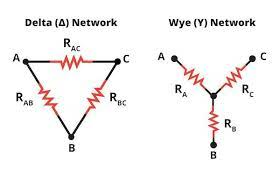
\includegraphics[scale=0.8]{figs/delta_wye.jpeg}
    \end{center}
\end{define}

For a $\wye$ configuration, there is an optional fourth wire, which serves as a neutral and is normally grounded. The ground wire present above many transmission lines are for fault protection and doesn't carry current under normal use.

There are four different types of three-phase transformer winding connections for transmission and distribution.
\begin{enumerate}
    \item $\wye - \wye$: for small current and high voltage
    \item $\Delta - \Delta$: for large currents and low voltages
    \item $\Delta - \wye$: for step-up transformers (ie generating stations)
    \item $\wye - \Delta$: for step-down transformers (ie at end of the transmission)
\end{enumerate}

\begin{figure}[H]
    \centering
    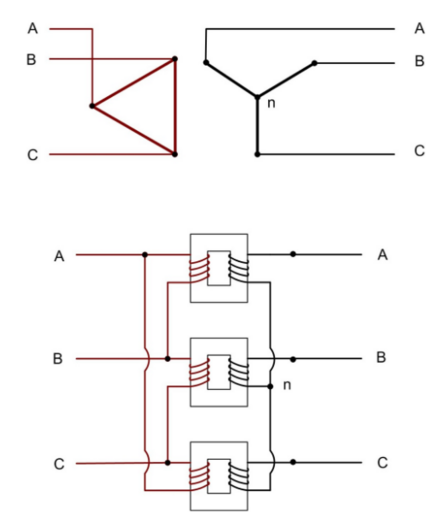
\includegraphics[scale=0.5]{figs/Delta-Wye_Transformer.png}
    \caption{This shows a delta-wye configuration across a transformer core. A practice transformer wouldn't have a different number of turns on each side.}
\end{figure}
\subsection{Single-Line Diagrams}

\begin{define}
    \textbf{Single-line diagram:} representation of an electrical system, providing a view of its components, interconnections, and electrical flow paths

    \textbf{Bus:} in an electrical system, this is a node where several line or several lines are connected. In power systems specifically, this is any garph node of the single-line diagram at which voltage, curernt, power flow or other quantities can be evaluated
\end{define}
Components on a single-line diagram
\begin{itemize}
    \item Power sources - includes generators, utility supplies and indicates their voltage levels and connection points to the electrical system
    \item Electrical Equipment - includes transformers, circuit breakers, switches, motors, and loads
    \item Bus arrangement - includes bus bars for power distribution at different voltage levels and shows how power is routed from one location to another
    \item Protective devices - includes fuses, circuit breakers, and relays
    \item Metering/instrumentation - includes metering devices (ammeter, voltmeter etc) and measuring points for monitoring/control
\end{itemize}

Individial components on a single-line diagram 

\textcolor{red}{do later: https://www.studyforfe.com/blog/fundamentals-of-single-line-diagrams/}

Bus Arrangement and Voltage Levels
\begin{define}
    Bus duct  
    \begin{itemize}
        \item Carries high currents between different electrical components and sections
        \item Ensures efficient power distribution and reduce
    \end{itemize}
    Transformer 
    \begin{itemize}
        \item Used to step down or setp up voltage levels
        \item Placed at locations to convert high-voltage power from the utility grid to lower voltages or to increase voltage for long-distance Transmission
        \item Winding figurations, type, kVA ratings, cool methods, and surge/lightning protection devices are listed
    \end{itemize}
    Voltage/current transformers (VT, CT)
    \begin{itemize}
        \item Used to measure voltage and current lvels for metering, protection, and control purposes
    \end{itemize}
\end{define}
\subsection{How to read AC \& DC Schematics and Power System Relaying}
\begin{concept}
    At its core, schematics graphically arrange the components of a system to emphasize the functional arrangement as opposed to the physical arrangement. Emphasizing function facilitates an understanding of how the system is supposed to operate and makes functional testing of systems much easier because it highlights relationships between elements.
\end{concept}

Other names for AC schematics include, AC Elementary Diagrams or Three Line Diagrams. DC Schematics are referred to as elementary wiring diagrams. The DC schematics depict the DC system and shows the protection and control functions of the equipment in the substation. Sometimes the control functions are supplied by AC and are included in the elementary diagram. Standards in the AC and DC schematic can differ slightly from utility to utility. Both of these schematics will include the rating for circuit elements like resistors, transformers etc.

Any depiction of reality by the single line diagram is on a large scale, it might show where major pieces of equipment are in relation to each other. On the other hand, though the AC and DC schematics still don’t show reality in every detail, they will contain information that will provide the link between the real depiction of the equipment seen in wiring diagrams and the almost purely functional depiction shown in the single line diagram.

Another vital function of the AC schematic is to show how the AC current and voltage circuits can be isolated for testing. For example, microprocessor delays might contribute to how secondary input quantities are measured as well as the directional sensitivity of specific elements.

\begin{concept}
    \textbf{AC and DC schematics} allow users to quickly trace a signal through the circuit and understand the function without regard to the actual physical wiring locations. Detail will include specific terminal numbers of devices and test switches to which connections are made. 
\end{concept}

\subsubsection{Common Practices}
\begin{enumerate}
    \item If complexity of the system requires it, the devices controlling the equipment.
    \item The DC circuit is usually shown with the positive bus closer to the top of the page and the negative bus closer to the bottom. The general layout of these drawings is that the DC source is usually shown at the left end of the drawing and the initiating contacts are shown above the operating elements. Control flow is generally shown so that the diagram is read from upper left to lower right.
\end{enumerate}

\subsubsection{DC Schematics and IEC 61850 Station Bus}
DC schematics: relay systems almost universally use DC for the controls; control ladder diagram or sometimes these are also referred to as elementary wiring diagrams.

IEC 61850 differs from other standards/protocols because it comprises several standards describing client/server and perr-to-peer communications, substation design and configuration, and testing. IEC 61850 provides a method for relay-to-relay interoperability between IEDs from different manufacturers. With the open architecture, it freely supports allocation of C37.2 device functions. The station bus described by IEC 61850 operates digitally over a secure Ethernet based network sending protecting relay messages called Generic Substation Events (GSE) or Generic Object Oriented Substation Events (GOOSE) between relays and other intelligent electronic devices (IEDs) on that network.

Because of this feature, it eliminates most dedicated control wiring that would normally be wired from relay-to-relay (i.e. a trip output contact from one relay to the input coil of another relay). Due to this digital communication between relays, a typical DC schematic diagram alone is not an adequate method for describing the system.
\subsection{High Voltage Direct Current}
% https://en.wikipedia.org/wiki/High-voltage_direct_current
Faults are defined as defects in the power system from current being distracted from the intended path. 
\subsection{SCADA}
SCADA stands for supervisory control and data acquisition. A SCADA system is a software-based application utilized within industrial manufacturing that controls an array of hardware components. Furthermore, as the acronym suggests, a SCADA system would contain a data component that would provide a historical overview of a system to the user. Such systems are employed within manufacturing environments in order to consolidate controls over multiple production lines, collect actionable data and to drive business decisions leading to process control and improvement.

The main goals of a SCADA system are listed:
\begin{enumerate}
    \item Control of manufacturing equipment on the plant floor
    \item Control and view of plant floor devices: Programmable Logic Controllers, sensors, valves, variable frequency drives, temperature probes, etc
    \item Display of real-time critical process information
    \item Acquisition, storage, and display of historical data
\end{enumerate}
 
\begin{figure}[H]
    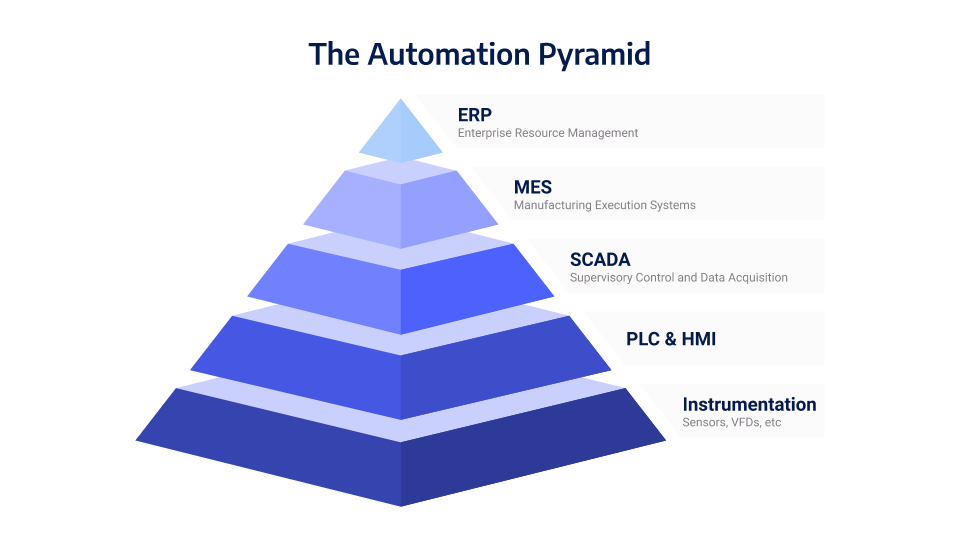
\includegraphics[scale=0.45]{figs/auto_pyramid.png}
    \caption{Automation pyramid to highlight how SCADA fits on here}
\end{figure}
A SCADA system would need to receive information from the PLC \& HMI to communicate with the instrumentation layer. Here PLC stands for programmable logic controller and HMI stands for human machine interface. The HIM system would display the current status of the system, alarms associated with the asset as well as a control screen used to make adjustments. An HMI would send the information to the PLC and vice versa; it would not interact with the instrumentation directly.

Control systems engineers to create a communication layer that would be instantiated within every PLC in order to pass data accordingly. An important infrastructure within this layer is the network. Although the PLC and HMI layers will require a network for data, the SCADA system would create an additional strain on the plant network due to the volume of data it will consume.
\begin{concept}
    SCADA refers to software while a PLC will refer to hardware. PLC as the brain of the production floor while SCADA connects to the PLC and processes this information.
\end{concept}

\subsubsection{Popular SCADA Software}
Different approaches to different components for each system results in each one being better suited for certain applications

Here are the following softwares mentioned:

Rockwell Automation - FactoryTalk View Site Edition and ThinManager
\begin{itemize}
    \item 
\end{itemize}

Siemens - WinCC RT Professional
\begin{itemize}
    \item 
\end{itemize}

Schneider Electric [AVEVA] - Wonderware
\begin{itemize}
    \item 
\end{itemize}

Inductive Automation - Ignition
\begin{itemize}
    \item 
\end{itemize}

\subsection{Substations Interview Questions and Answers}

\textbf{What are the merits of indoor and outdoor substations?}

Merits of indoor substations
\begin{itemize}
    \item Less requirement of space
    \item Less maintainance 
    \item Less control cable length
    \item Protection from lightning
    \item Flexibility in installation
    \item No dust and dirt
\end{itemize}

\subsection{\href{https://peguru.com/quiz-substation-engineering/}{Substation Engineering Quiz}}
    \begin{enumerate}
        \item \textcolor{blue}{You are building an interconnect station, tying wind farm generation to the power grid. At the substation, the sources are tied through a tie-breaker. Which device would you install to make sure the sources are synchronized?} A synchronization check is done using a relay. It needs low voltage input (from both sides), obtained using a voltage transformer a.k.a. instrument transformer.
    \end{enumerate}

\newpage
\section{Sources}
\begin{itemize}
    \item Chapter 1
    \begin{enumerate}
        \item \href{https://www.youtube.com/watch?v=hRAyfJLZnC0&list=PLmK1EnKxphinxBub5hL0ZoJXWoqjkGE19}{katkimshow} Youtube Channel playlist "Introduction to Power Electronics (2023) for most of the introduction
        \item \href{https://www.youtube.com/watch?v=tClE8s6RZdg}{Why your Function Generator's output voltage reading can be wrong}: section 1.1.1
        \item \href{https://www.allaboutcircuits.com/textbook/alternating-current/chpt-11/true-reactive-and-apparent-power/}{True, Reactive, and Apparent Power}: section 1.2 examples
    \end{enumerate}

    \item Chapter 2
    % include impedance matching here: https://www.analog.com/en/resources/glossary/impedance-matching.html
    
    \item Transmission and Distribution
    \begin{enumerate}
        \item \href{https://en.wikipedia.org/wiki/Three-phase_electric_power}{Three-phase electric power}: Three phase power section
        \item \href{https://electronics.stackexchange.com/questions/185308/why-three-phase-power-why-not-a-higher-number-of-phases}{Why three-phase power? Why not a higher number of phases?}
        \item \href{https://circuitglobe.com/types-of-faults-in-power-system.html}{Types of Faults in Power System}
        \item AC DC Schematics
        \begin{enumerate}
            \item \href{https://electrical-engineering-portal.com/ac-dc-schematics-protection-control-relaying}{Protection \& Control Relaying Schematics}
            \item \href{https://www.pes-psrc.org/kb/report/047.pdf}{PSRC I5 Schematic Representation of Power System Relaying}
            \item \href{https://www.daltco.com/sites/daltco.com/files/resource/schneider-wiring-diagram-book.pdf}{Wiring diagram book}
        \end{enumerate}
        \item SCADA 
        \begin{enumerate}
            \item \href{https://www.solisplc.com/scada}{An Introduction to Supervisory Control \& Data Acquisition (SCADA)}
            \item \href{https://www.euci.com/event_post/scada-fundamentals-energy-management-system/}{SCADA 101: Fundamentals with a Focus on Energy Management System (EMS)}
        \end{enumerate}
        \item \href{https://www.eeeguide.com/substations-interview-questions-and-answers/}{Substation Interview QA}
    \end{enumerate}

    \item unfiled
    \begin{enumerate}
        \item \href{https://eepower.com/technical-articles/understanding-impedance-matching/#}{Understanding Impedance Matching}
    \end{enumerate}
\end{itemize}

THIS IS A TODO U LAZY MF RE FUCKING ORGANIZE TIHS MESS AND GO THROUGH THESE LINKS TO EXTRACT INFO
\begin{enumerate}
    \item \href{https://www.youtube.com/watch?v=WujIkCgawFI&list=PLmK1EnKxphinxBub5hL0ZoJXWoqjkGE19&index=11}{link}
    \item \href{https://www.youtube.com/watch?v=jgh0TNfx0gQ}{link}
    \item \href{https://eshop.se.com/in/blog/post/difference-between-active-power-reactive-power-and-apparent-power.html#}{link}
    \item \href{https://www.allaboutcircuits.com/textbook/alternating-current/chpt-11/true-reactive-and-apparent-power/}{link}
    \item \href{https://laurenselectric.com/commercial-services/understanding-power-factor/}{link}
    \item \href{https://www.eeeguide.com/substations-interview-questions-and-answers/}{link}
    \item \href{https://circuitglobe.com/types-of-faults-in-power-system.html}{link}
    \item \href{https://peguru.com/2019/08/voltage-transformer/}{link}
    \item \href{https://www.pes-psrc.org/kb/report/047.pdf}{link}
    \item \href{https://electrical-engineering-portal.com/download-center/books-and-guides/relays}{link}
    \item \href{https://www.studyforfe.com/blog/fundamentals-of-single-line-diagrams/}{link}
    \item \href{https://eepower.com/technical-articles/calculating-the-turns-ratio-of-a-transformer/}{link}
    \item \href{https://eepower.com/power-electronics-textbook/vol-i-electrical-power-systems-design/chapter-5-impedance-matching-and-power-transfer/understanding-electrical-transformers/#}{link}
\end{enumerate}

\end{document}